\pdfoutput=1
\pdfcompresslevel=9
\pdfinfo
{
    /Author (Autor)
    /Title (Tytuł pracy magisterskiej)
    /Subject (Bioinformatyka)
    /Keywords (DNAASM)
}
%\documentclass[a4paper,polish,onecolumn,oneside,floatssmall,11pt,titleauthor,wide,openright]{mwrep}
%\usepackage[scale={0.7,0.8},paper=a4paper,twoside]{geometry}
\documentclass[a4paper,onecolumn,twoside,openright,11pt,wide,floatssmall]{mwrep}
% \usepackage{polish}
\usepackage{amsmath}
\usepackage{amsfonts}
\usepackage{amssymb}
\usepackage{amsthm}
\usepackage{bookman}
\usepackage{algorithm}
\usepackage{algpseudocode}
\usepackage{geometry}
\usepackage{placeins}
%\usepackage{slashbox}
\usepackage[utf8x]{inputenc}
\usepackage[T1]{fontenc}
\usepackage{footnote}
\usepackage{enumerate}
% \usepackage{fancyvrb}
% \usepackage{t1enc}
% \usepackage[pdftex, bookmarks]{hyperref}
\usepackage[pdftex, bookmarks=false]{hyperref}

\floatname{algorithm}{Algorytm}
\renewcommand{\algorithmicforall}{\textbf{for each}}

\usepackage{caption}
%\usepackage[vlined]{algorithm2e}

\def\url#1{{ \tt #1}}

\usepackage{listings}


\usepackage{fancyhdr}
\pagestyle{fancy}
\fancyhf{}
\fancyhead[CE,CO]{\leftmark}
\fancyfoot[LE,RO]{\thepage}
\usepackage[toc,page]{appendix}

\fancypagestyle{plain}{%
\fancyhf{}%
\fancyfoot[LE,RO]{\thepage}}

% marginesy
\textwidth\paperwidth
\advance\textwidth -55mm
\oddsidemargin-0.9in
\advance\oddsidemargin33mm
\evensidemargin0.9in
\advance\evensidemargin-33mm

\topmargin -1in
\advance\topmargin 25mm
\setlength\textheight{48\baselineskip}
\addtolength\textheight{\topskip}
\marginparwidth15mm

\clubpenalty=10000 % to kara za sierotki
\widowpenalty=10000 % nie pozostawia wdów
\brokenpenalty=10000 % nie dzieli wyrazów pomiędzy stronami
\sloppy

\tolerance4500
\pretolerance250
\hfuzz=1.5pt
\hbadness1450

\linespread{1.5} %interlinia
% ŻYWA PAGINA
\renewcommand{\chaptermark}[1]{\markboth{\scshape\small\bfseries \
#1}{\small\bfseries \ #1}}
\renewcommand{\sectionmark}[1]{\markboth{\scshape\small\bfseries\thesection.\
#1}{\small\bfseries\thesection.\ #1}}
\renewcommand{\headrulewidth}{0.5pt}
\renewcommand{\footrulewidth}{0.pt}
%%\pagestyle{uheadings}

\usepackage[pdftex]{color,graphicx}
\usepackage[polish]{babel}

% \textheight232mm
% \setlength{\textwidth}{\textwidth}
% \setlength{\oddsidemargin}{\evensidemargin}
% \setlength{\evensidemargin}{0.3cm}
\usepackage[sort, compress]{cite}

% definicje komand todo
\newcommand\todo[1]{\textcolor{red}{#1}}
\newcommand\mockup[1]{\textcolor{blue}{#1}}

%\usepackage{multibib}
%\newcites{bk,st,doc,web}{Książki i~artykuły,Standardy i~zalecenia,Dokumentacja produktów,Publikacje i~serwisy internetowe}

\theoremstyle{definition}
\newtheorem{defn}{Definicja}[chapter]
\newtheorem{conj}{Teza}[section]
\newtheorem{conjmain}{Teza}
\newtheorem{exmp}{Przykład}[chapter]

\theoremstyle{plain}% default
\newtheorem{thm}{Twierdzenie}[section]
\newtheorem{lem}[thm]{Lemat}
\newtheorem{prop}[thm]{Hipoteza}
\newtheorem*{cor}{Wniosek}

\theoremstyle{remark}
\newtheorem*{rem}{Uwaga}
\newtheorem*{note}{Uwaga}
\newtheorem{case}{Przypadek}[chapter]

\definecolor{ListingBackground}{rgb}{0.95,0.95,0.95}

\begin{document}

% kody źródłowe wplatane w tekst
\lstdefinestyle{incode}
{
basicstyle={\footnotesize},
keywordstyle={\bf\footnotesize\color{blue}},
commentstyle={\em\footnotesize\color{magenta}},
numbers=left,
stepnumber=5,
firstnumber=1,
numberfirstline=true,
numberblanklines=true,
numberstyle={\sf\tiny},
numbersep=10pt,
tabsize=2,
xleftmargin=17pt,
framexleftmargin=3pt,
framexbottommargin=2pt,
framextopmargin=2pt,
framexrightmargin=0pt,
showstringspaces=true,
backgroundcolor={\color{ListingBackground}},
extendedchars=true,
% title=\lstname,
captionpos=b,
% abovecaptionskip=1pt,
% belowcaptionskip=1pt,
frame=tb,
framerule=0pt,
}

% kody źródłowe z podpisem
\lstdefinestyle{outcode}
{
basicstyle={\footnotesize},
keywordstyle={\bf\footnotesize\color{blue}},
commentstyle={\em\footnotesize\color{magenta}},
numbers=left,
stepnumber=5,
firstnumber=1,
numberfirstline=true,
numberblanklines=true,
numberstyle={\sf\tiny},
numbersep=10pt,
tabsize=2,
xleftmargin=17pt,
framexleftmargin=3pt,
framexbottommargin=2pt,
framextopmargin=2pt,
framexrightmargin=0pt,
showstringspaces=true,
backgroundcolor={\color{ListingBackground}},
extendedchars=true,
% title=\lstname,
captionpos=b,
% abovecaptionskip=1pt,
% belowcaptionskip=1pt,
frame=tb,
framerule=0.1pt,
}

%\counterwithin{exmp}{chapter}
%\counterwithout{exmp}{section}
\renewcommand*\lstlistingname{Wydruk}
\renewcommand*\lstlistlistingname{Spis wydruków}

\pagenumbering{roman}
\renewcommand{\baselinestretch}{1.0}
\raggedbottom

% todo odkomentować strony tytulowe !
% 
\begin{titlepage}
    % Strona tytułowa


    % Życiorys
    \newpage\thispagestyle{empty}
    \begin{tabular}{p{5cm} p{12cm}}
    \begin{minipage}{5cm}
    \center
    %% \includegraphics[height=6.5cm,width=4.5cm]{img/ja.png}
    \end{minipage}
    &
    \begin{minipage}{12cm}
    \begin{flushleft}
    \par\noindent\vspace{0\baselineskip}
    \begin{tabular}[h]{l l}
    {\normalsize\it Specjalność:} & Informatyka -- \\
    & Systemy Informacyjno Decyzyjne \\
    \end{tabular}
    \par\noindent\vspace{1\baselineskip}
    \begin{tabular}[h]{l l}
    {\normalsize\it Data urodzenia:} & {\normalsize 03.04.1992}
    \end{tabular}
    \par\noindent\vspace{1\baselineskip}
    \begin{tabular}[h]{l l}
    {\normalsize\it Data rozpoczęcia studiów:} & {\normalsize 20.02.2016}%1 października 2012 r.}
    \end{tabular}
    \par\noindent\vspace{1\baselineskip}
    \end{flushleft}
    \end{minipage}
    \end{tabular}
    \vspace*{0\baselineskip}
    \begin{center}
	{\large\bfseries Życiorys}\par\bigskip
    \end{center}
	\mockup{
	Urodziłem się 3 kwietnia 1992 roku w~Kielcach. W~2008 roku rozpocząłem naukę w~II Liceum Ogólnokształcącym im. Jana Śniadeckiego w~Kielcach, w~klasie o~podstawie programowej w~zakresie rozszerzonym z~matematyki, informatyki, fizyki i~astronomii . W~2011 roku uzyskałem wykształcenie średnie oraz świadectwo dojrzałości... 
	}
    \indent

    \par
    \vspace{2\baselineskip}
    \hfill\parbox{15em}{{\small\dotfill}\\[-.3ex]
    \centerline{\footnotesize podpis studenta}}\par
    \vspace{1\baselineskip}
    \begin{center}
 	{\large\bfseries Egzamin dyplomowy} \par\bigskip\bigskip
    \end{center}
    \par\noindent\vspace{1.0\baselineskip}
    Złożył egzamin dyplomowy w dn. \dotfill
    \par\noindent\vspace{1.0\baselineskip}
    Z wynikiem \dotfill
    \par\noindent\vspace{1.0\baselineskip}
    Ogólny wynik studiów \dotfill
    \par\noindent\vspace{1.0\baselineskip}
    Dodatkowe wnioski i uwagi Komisji \dotfill
    \par\noindent\vspace{1.0\baselineskip}
    \dotfill

    % Streszczenie po polsku
    \newpage\thispagestyle{empty}
    \vspace*{2\baselineskip}
    \begin{center}
	{\large\bfseries Streszczenie}\par\bigskip
	\vspace*{2\baselineskip}
    \end{center}

    \itshape
    \todo{todo}
    \vspace*{3\baselineskip}

    \noindent{\bf Słowa kluczowe}: {\itshape \todo{todo.}}
    %\par
    %\vspace{4\baselineskip}
    
    % Streszczenie po angielsku
    \newpage\thispagestyle{empty}
    \vspace*{2\baselineskip}
    \begin{center}
	{\large\bfseries Abstract}\par\bigskip
	\vspace*{2\baselineskip}
    \end{center}
    \noindent{\bf Title}: {\itshape \todo{XXX}}\par
    \vspace*{1\baselineskip}
    \itshape
    \todo{XXX}
    \vspace*{3\baselineskip}

    \noindent{\bf Key words}: {\itshape \todo{XXX}.}

\end{titlepage}

% ex: set tabstop=4 shiftwidth=4 softtabstop=4 noexpandtab fileformat=unix filetype=tex spelllang=pl,en spell:


%\newpage\null\thispagestyle{empty}\newpage

% % Podziękowania
\newpage\thispagestyle{empty}



\tableofcontents
% \addcontentsline{toc}{chapter}{{Przedmowa1}{vii}}{vii}

% \chapter*{Spis tablic, rysunków i~wydruków}
% \listoftables
% \listoffigures
% \listofalgorithms
% \lstlistoflistings

%\setlength{\baselineskip}{7mm}
\newpage
\pagenumbering{arabic}
\raggedbottom{}
\setcounter{page}{1}



\chapter{Wstęp}
\label{section:wstep}

\section{Cel i zakres pracy}
\label{section:cel_i_zakres_pracy}

\subsection{Hipotezy}

\begin{enumerate}[I.]
	\item \textit{
		Można zaproponować strukturę bazy danych do przechowywania danych opisujących genomy, taką że będzie ona elastyczna, łatwa w modyfikacji, uniezależniona od semantyki przechowywanych struktur biologicznych.
		} \\
	\todo{krótki opis}
	
	\item \textit{
		Można dostarczyć abstrakcję widoków na dane genetyczne, umożliwiające analizę danych z różnych perspektyw w kontekście licznych zbiorów
		danych genetycznych.
		} \\
	\todo{krótki opis}
	
	\item \textit{
		Można dostarczyć aplikację do przechowywania i analizy genomów, która w~przystępny sposób umożliwi przeglądanie sekwencji genetyczych bez konieczności posiadania wydajnej maszyny klienckiej. 
		} \\
	\todo{krótki opis}
	
\end{enumerate}

\subsection{Plan badań}
-genom ogorka \\
-baza danych generycza \\
-algorytmy \\
-wygoda uzytkownika \\
-wydajne przegladanie \\

\section{Układ pracy}
\label{section:uklad_pracy}

\section{Przegląd literatury}

\chapter{Biologiczna potrzeba}
\label{section:biologiny_wstep}

\section{Bioinformatyka w praktyce}
\subsection{medycyna}
\subsection{farmaceutyka}
\subsection{kryminalistyka}
\subsection{sądownictwo}
\subsection{rolnictwo}
\subsection{archeologia}

\section{Bioinformatyka w ujęciu algorytmicznym}
\subsection{bazy danych}
\subsection{big data}
\subsection{uczenie maszynowe}
\subsection{metody optymalizacji}
\subsection{teoria grafów}

\section{Problemy bioinformatyki}
-niekontynuowane projekty
-dane bazują na eksperymentach, błędy propagujące się
-wiele różnych standardów, niekompatybilne
-nieinformatyczni biolodzy
-sposoby finansowania nauki

\section{Centralny dogmat bioinformatyki}
-dna, rna, białko
-informacja genetyczna
-struktura molekularna
-funkcja biochemiczna
-fenotyp

\section{Rozwój bioinformatyki}
\subsection{wcześniej}
\subsection{obecnie}
\subsection{w przyszłości}

\section{Genom ogórka}
-sggw


\chapter{Projekt i implementacja}


\section{Architektura}

Przeglądarka została zaimplementowana w wielowarstwowej architekturze klient-serwer.
Kod został podzielony na moduły, aby jak najbardziej oddzielić od siebie niezależne fragmenty aplikacji zachowując przy tym dobre praktyki programistyczne.
Rozróżniamy w pracy 3 główne warstwy odpowiadające za:
\begin{itemize}
	\item prezentację
	\item obsługę danych
	\item logikę biznesową
\end{itemize}

\subsection*{BioWeb}

BioWeb jest środowiskiem aplikacyjnym, w którym zostało stworzonych wiele aplikacji przetwarzających dane genetyczne \cite{article:bioweb}.
Programy operujące na obszernych zbiorach genetycznych wymagają architektury zapewniającej m.in. przenośność, elastyczność i wysoką wydajność nie rezygnując jednocześnie z interaktywnego interfejsu użytkownika.
Zaspokojenie ww. wymagań możliwe jest dzięki połączeniu ze sobą w jednym projekcie języków kompilowanych i interpretowanych.
Zastosowanie architektury BioWeb przyspiesza sam proces wytwarzania oprogramowania poprzez podejście zalecające implementację jedynie modułów obliczeniowych w językach niskiego poziomu (C++), natomiast część serwerową i kliencką, które nie są wąskimi gardłami, w językach interpretowanych takich jak Python i Javascript.
Innymi słowy - moduły nie wymagające ponad przeciętnej wydajności, które można stworzyć szybciej, implementowane są w językach wyższego poziomu a moduły zasobożerne są w językach niskiego poziomu. Odpowiedni dobór konkretnych technologii dał możliwość wygodnego połączenia ww. technik.
Na rysunku \todo{[link]} zamieszony został schemat struktury aplikacji.
\\
\todo{[rysunek schematu - trójwarstwowa aplikacja ze schematem technologii.]}


\subsection*{Klient, warstwa prezentacji}
Moduł klienta znajdujący się w warstwie prezentacji możemy zaliczyć do grupy klientów cienkich.
Odpowiada on za ilustrowanie danych pobranych z serwera wykonując operacje renderowania elementów graficznych oraz zapewnia interaktywną komunikację użytkownika z systemem.
W obecnych czasach, praktycznie każdy komputer stacjonarny a nawet urządzenia mobilne posiadają stosunkowo dużą moc obliczeniową pozwalającą na proste przetwarzanie.
Realizując projekt, zastosowano podejście, w którym odpowiedzialność za operacje takie jak walidacja danych, generowanie rysunków czy animacje pozostają na barkach modułu klienckiego. 
Tym samym, odciążony zostaje serwer, przez co podwyższamy jego możliwości wydajnościowe co sprowadza się do zwiększenia potencjalnej liczby jednocześnie obsługiwanych użytkowników.

Do implementacji warstwy prezentacji zostały użyte technologie webowe, wykorzystujące jako środowisko uruchomieniowe przeglądarkę internetową. Użytkownikowi wystarczy jedynie maszyna z dostępem do internetu i nowoczesną przeglądarką internetową wpierająca HTML5. 
Klient może być uruchomiony na dowolnym popularnym systemie operacyjnym \mbox{(Linux/Mac/Windows)} i zwolniony jest z potrzeby aktualizowania aplikacji - wszystkie moduły ładowane są podczas inicjacji przeglądarki genomu.

\subsection*{Serwer - warstwa trwałości i przetwarzania}
Serwer jest przenośny, wykorzystuje technologie dające się uruchomić na najpopularniejszych platformach komputerowych - Unix, Windows.
System pozwala na równoległą obsługę wielu użytkowników jednocześnie.
W celu zwiększenia wydajności aplikacja daje się stosunkowo łatwo skalować horyzontalnie i wertykalnie.
Wpływ na szybkość przetwarzania żądań, głównie ma klasa zastosowanego sprzętu komputerowego.
Jego główne zadania to gromadzenie danych, udostępnienie ich dla aplikacji klienckiej poprzez API, przechowywanie stanu przeglądarki, wykonywanie zadań przeszukiwania genomu.

\section{Wykorzystane technologie}
Python jest głównym językiem programowania używanym w przeglądarce.
Jest interpretowany, wspiera wiele paradygmatów programowania, uważany jest jako prosty do nauki, posiada rozbudowaną bibliotekę standardową i jest mocno wspierany przez społeczność. 
Aplikacje pisane w nim są przenośne i szybkie zarazem, ponieważ wiele bibliotek pod spodem jest zaimplementowanych w C/C++.

Algorytmy do wyszukiwania sekwencji, zostały zaimplementowane w języku C++ i zintegrowane z częścią serwerową za pomocą biblioteki \textit{BoostPython}.
Biblioteka ta stworzona została aby szybko i łatwo eksportować C++ do Pythona.
Jest tak zaprojektowana, aby była minimalnie inwazyjna dla kodu C++ - w większości przypadków nie ma konieczności w żaden sposób zmieniać klas C++ aby używać ich z \textit{BoostPython}.

Aby uprościć standardowe czynności związane z pisaniem aplikacji webowej wykorzystany został popularny framework pythonowy - Django. 
Automatyzuje on wiele zadań związanych z obsługą żądań HTTP (Django REST Framework), dostarcza panel administracyjny, system cache'owania, serwer do testowania aplikacji i wiele innych.
Kluczową dostarczoną funkcjonalnością jest maper obiektowo relacyjny ORM\footnote{ang. Object Relational Mapping.}, który w wygodny sposób daje nam dostęp do danych zgromadzonych w bazie danych bez potrzeby pisania niekiedy skomplikowanych zapytań SQL.
Jako system bazodanowy użyty został PostgreSQL - jeden z najpopularniejszych systemów relacyjnych o otwartym kodzie źródłowym.

Jako serwer WWW wykorzystany został Nginx, który z Django łączy się za pośrednictwem serwera HTTP Gunicorn implementującego interfejs WSGI\footnote{ang. Web Server Gateway Interface.}.

Podstawą części wizualizacyjnej, dostarczającej graficzny interfejs użytkownika (GUI\footnote{ang. Graphical User Interface}) jest język HTML5 wraz z JavaScriptem.
Element ,,canvas'' pozwala na dynamiczne, skryptowe renderowanie kształtów i obrazów bitmapowych bez dodatkowych wtyczek - został użyty do odrysowywania głównego widoku mapy genomu.
Aby ułatwić zadania towarzyszące tworzeniu aplikacji w modelu SPA\footnote{ang. Single Page Application}, wykorzystany został framework \textit{AngularJS} oparty o wzorzec projektowy MVC\footnote{ang. Model View Controller}.
Angular jest otwartoźródłowym projektem wydanym i rozwijanym przez firmę \textit{Google}.
Bardzo pomocny przy implementacji wartwy prezentacji okazał się również framework CSS\footnote{ang. Cascading Style Sheets} \textit{Bootstrap}, który ułatwił stylizację komponentów wyświetlanych na stronie.

Fragmenty kodu odpowiedzialne za budowanie aplikacji, uruchamianie jej w różnych konfiguracjach, kompilację modułów obliczeniowych itp. wykorzystują narzędzie \textit{SCons}.
Pliki konfiguracyjne mają formę skryptów pythonowych, natomiast sama funkcjonalność narzędzia pod wieloma względami przypomina tradycyjny program powłoki systemowej, automatyzujący np. proces kompilacji programów - \textit{GNU make}.

\begin{figure}[h]
	\centering
	
\includegraphics[width=1\textwidth]{img/loga.png}
	\caption{Technologie wykorzystane w projekcie.}
	\vspace{-0.5cm}
	\label{img:technologie}
\end{figure}


\section{Struktura projektu}
\todo{todo: obrazek z drzewem projektu\\}
W niniejszym rozdziale przybliżę strukturę plików i folderów w projekcie oraz wyszczególnię ważniejsze fragmenty kodu.
Zaimplementowana aplikacja została podzielona na następujące moduły:

\subsection*{build\_tools}
Zawiera klasy wykorzystywane do budowania aplikacji, pliki konfiguracyjne:


\begin{itemize}
	\item \textit{requirements.txt} - spis bibliotek pythonowych, które zostaną zainstalowane w wyizolowanym środowisku \textit{virtualenv}.
	\todo{todo: dodać link do opisu pliku SCons}
	
	\item \textit{deploy\_conf\_files} - folder zawierający szablon pliku konfiguracyjnego serwera www \textit{nginx}, wykorzystywany przy produkcyjnym budowaniu aplikacji.
	\todo{todo: dodać link do opisu pliku SCons}
	
	\item \textit{build.AppBuilder} - klasa umożliwiająca zarządzanie plikiem konfigurującym proces budowania, tworzenie struktury folderów projektu, utworzenie środowiska \textit{virtualenv} wraz z pobraniem i zainstalowaniem niezbędnych bibliotek pythonowych, pobranie i wypakowanie plików zawierających dane dotyczące genomu ogórka, które wykorzystywane są podczas inicjacji bazy danych.
	
	\item \textit{deploy.Deployer} - klasa pozwalająca renderować plik konfiguracyjny serwera www \textit{nginx}, generować sekretny klucz \textit{Django}, konfigurować ustawienie \textit{Django ALLOWED\_HOSTS} niezbędne do prawidłowego działania serwera.
\end{itemize}

\subsection*{functional\_tests}
Zawiera sterownik do silnika przeglądarki \textit{Chrome} oraz testy funkcjonalne wykorzystujące bibliotekę do testowania webowych aplikacji - \textit{Selenium}.

\subsection*{zpr}
Zawiera główne ustawienia \textit{Django} (settings.py) oraz korzeń API HTTP aplikacji (urls.py).

\subsection*{zpr/database}
Zawiera skrypty służące do parsowania danych biologicznych pozyskanych od SGGW, narzędzia do obrabiania tych danych, tj. ekstrahowania informacji, przygotowywania struktur pomocniczych, grupowania, filtrowania, zliczania, sortowania oraz finalnie - generowania ciągów chromosomów po odrzuceniu błędnych, niespójnych danych.

\subsection*{zprapp}
Główny folder aplikacji, zawiera moduły logiki i prezentacji.
Bezpośrednio w folderze znajdują się m.in. pliki widoków API, serializerów, trasowania url, panelu administracyjnego, schematu bazy danych, testów jednostkowych.

\subsection*{zprapp/calc}
Zawiera algorytmy wyszukiwania podciągów zaimplementowane w języku \textit{C++}: \textit{Knutha-Morrisa-Pratta}, \textit{Boyera-Moore'a}, \textit{Smitha-Watermana}, \textit{BLAST} oraz ich interfejsy pozwalające na wywołanie kodu bezpośrednio z poziomu \textit{Pythona}. Algorytmy zostały zaimplementowane przez \textit{Piotra Róża}.

\subsection*{zprapp/templates/zprapp}
Zawiera pliki HTML dynamicznie renderowane w przeglądarce internetowej podczas użytkowania aplikacji.

\subsection*{zprapp/static/zprapp}
Zawiera biblioteki Javascriptowe wraz ze stylami CSS wykorzystywane po stronie frontendu.
Tutaj została zaimplementowana większość kodu kontrolerów Angularowych.
W folderze \textit{lang} obecne są również pliki zawierające tłumaczenia słów w dwóch językach - angielskim i polskim.
Aplikację w prosty, nieinwazyjny sposób można rozszerzyć o więcej języków.

\subsection*{zprapp/contrib}
Lokalizacja zawierają funkcje i klasy wykorzystywane m.in. do pomiarów i porównania szybkości algorytmów oraz łączenia ciągów podsekwencji w dłuższe fragmenty.


\section{Baza danych}

\section{Algorytmy}

\section{Sekwencje ogórka}

\section{Interfejs użytkownika}

\section{Instrukcja uruchomienia aplikacji}
W celu zautomatyzowania budowy, kompilacji oraz konfiguracji aplikacji zostało wykorzystane narzędzie \textit{Scons}.
Aby zbudować i uruchomić część serwerową przeglądarki genomów w środowisku Linux z rodziny \textit{Debian}, zaleca się wykonać następujące czynności:
\begin{enumerate}
	\item zainstalować bazę danych \textit{PostgreSQL} w wersji 9.5
	\item zainstalować język Python w wersji 2.7 wraz menadżerem paczek \textit{pip} i środowiskiem virtualenv
	\item zainstalować bibliotekę \textit{Boost} w wersji 1.64
\end{enumerate}
Powyższe zadania można wykonać poleceniami:

\begin{spverbatim}
	apt-get install libpq-dev python-dev python-pip scons postgresql nginx
	pip2 install virtualenv
	tar --bzip2 -xf /path/to/boost_1_64_0.tar.bz2 ./bootstrap.sh --with-python=python ./b2 install
\end{spverbatim}

\begin{enumerate}[resume]
	\item utworzyć użytkownika \textit{zpr} o haśle \textit{zpr}
	\item utworzyć bazy danych \textit{zpr} oraz \textit{ogorek\_roboczy}
\end{enumerate}
Powyższe zadania można wykonać poleceniami:

\begin{spverbatim}
	sudo -u postgres createuser --superuser --createdb --createrole zpr 
	sudo -u postgres psql -c "alter user zpr with encrypted password 'zpr';"
	sudo -u postgres createdb -O zpr zpr 
	sudo -u postgres createdb -O zpr ogorek_roboczy
\end{spverbatim}

\begin{enumerate}[resume]
	\item przetestować połączenie z bazą danych poleceniem\\
	\verb|psql zpr -U zpr|\\
	w przypadku pojawiającego się błędu\\
	\verb|psql: FATAL: Peer authentication failed for user "zpr""|
	należy w pliku \textit{/etc/postgresql/9.5/main/pg\_hba.conf} w linijce \textit{local all all peer} zamienić \textit{peer} na \textit{md5}, następnie zrestartuj serwer poleceniem\\
	\verb|#/etc/init.d/postgresql restart|
	
	\item zbudować program wraz ze środowiskiem poleceniem \verb|scons|
	
	\item wczytać bazę danych \textit{ogorek\_roboczy} poleceniem\\
	\verb|scons restore_ogorek_roboczy=1|
	
	\item zbudować główną bazę danych poleceniem \verb|scons build_db=1|
	
	\item w celu konfiguracji produkcyjnej serwera www \textit{nginx} wykonać:\\
	\verb|sudo scons build_deploy=1|\\
	Należy pamiętać aby w pliku \textit{SConstruct} ustawić odpowiednio zmienne, w szczególności \textit{WWW\_SRV\_HOST}.
	W razie błędu \textit{HTTP 400}, należy sprawdzić czy w pliku \textit{settings.py}, w zmiennej \textit{ALLOWED\_HOSTS} jest prawidłowo wpisana wartość \textit{WWW\_SRV\_HOST}.
	
	\item wygenerować nowy klucz zabezpieczeń \textit{Django} poleceniem:
	\verb|new_secret_key=1|\\
	Klucz powinien pozostać taki sam w poszczególnych wdrożeniach.
	
	\item uruchomić serwer lokalnie bądź produkcyjnie poleceniami odpowiednio:\\
	\verb|scons run=l| lub \verb|scons run=p|\\
	Jeśli serwer www nie serwuje prawidłowo plików statycznych należy sprawdzić uprawnienia dostępu do folderu \textit{static}
\end{enumerate}







\chapter{Wyniki}

\section{Baza danych}
-znaczenie danych

\section{Sekwencje ogórka}
\todo{tabela z wynikami \ref{tab:genome_stat}}

\begin{table}
	\centering
	\begin{tabular}{|c||r|r|r|c|} \hline
		\textbf{Chromosom}    & Długość [Mbp] & Liczba & Zmapowana & Zmapowana \\
		& & zmapowanych contigów & długość [bp] & długość [\%] \\
		\hline
		\textbf{1}             & 55                 &  22                 &  32970425          & 59.9\%               \\
		\textbf{2}             & 44                 &  13                 &  23992470          & 52.2\%               \\
		\textbf{3}             & 65                 &  14                 &  39532546          & 60.8\%               \\
		\textbf{4}             & 61                 &  15                 &  24781874          & 40.6\%               \\
		\textbf{5}             & 49                 &  22                 &  26573846          & 54.2\%               \\
		\textbf{6}             & 42                 &  19                 &  29507078          & 70.2\%               \\
		\textbf{7}             & 52                 &  11                 &  18951584          & 36.4\%               \\
		\hline
		$\mathbf{\Sigma}$      &368                 & 116                 & 196309823          &  53.3\%              \\
		\hline
	\end{tabular}
	\caption{Chromosome statistic for mapped contigs of Nothern European cucumber genome.
		The length of the chromosomes and length of the genome described in~Chen's studies\cite{article:reevaluation_in_cucumber} was used.}
	\label{tab:genome_stat}
\end{table}

\section{API}

\section{Algorytmy}
Porównanie ze sobą dwóch sekwencji nie może polegać na zwykłej analizie ciągów tekstowych, ponieważ porównując ciągi musimy brać pod uwagę ich podłoże ewolucyjne. Chcemy sprawdzić na ile podobna jest jedna sekwencja do drugiej, analizując możliwość ewolucyjnego przekształcenia pierwszej w drugą. 
\todo{porównanie, komentarz}

\begin{figure}[h]
	\centering
	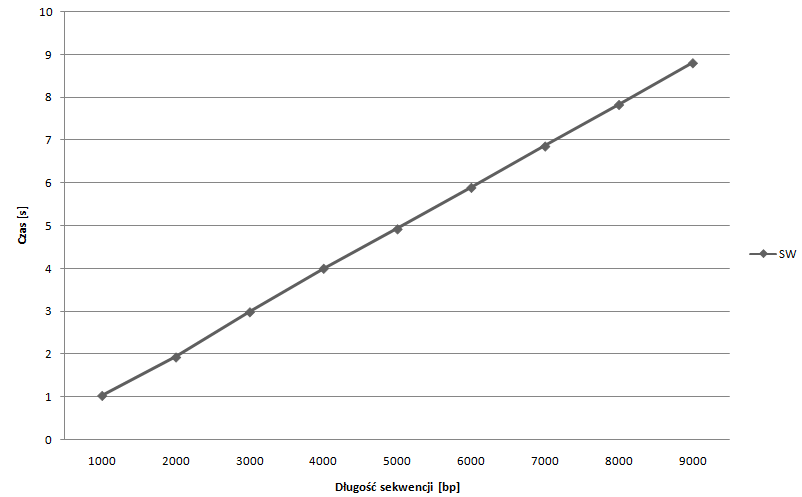
\includegraphics[width=1\textwidth]{img/sm-sekwencja-zmienna.png}
	\caption{\todo{opis - zmienna sekwencja}}
	\label{img:sm-sekwencja-zmienna}
\end{figure}

\begin{figure}[h]
	\centering
	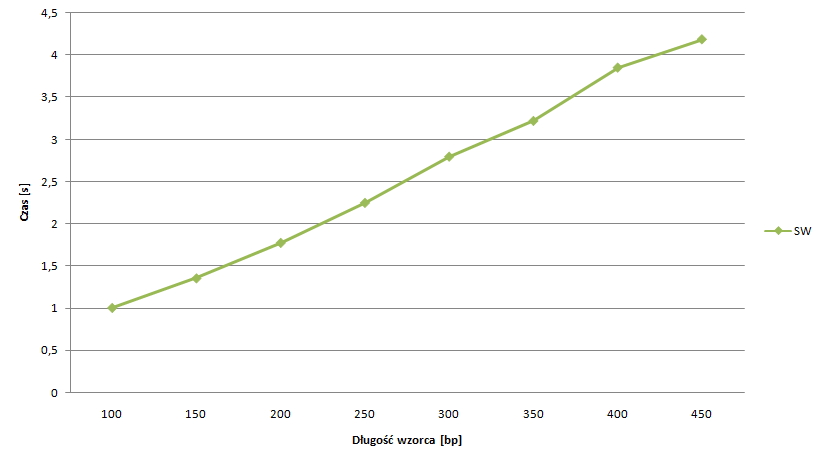
\includegraphics[width=1\textwidth]{img/sm-wzorzec-zmienny.png}
	\caption{\todo{opis - zmienny wzorzec}}
	\label{img:sm-wzorzec-zmienny}
\end{figure}

\begin{figure}[h]
	\centering
	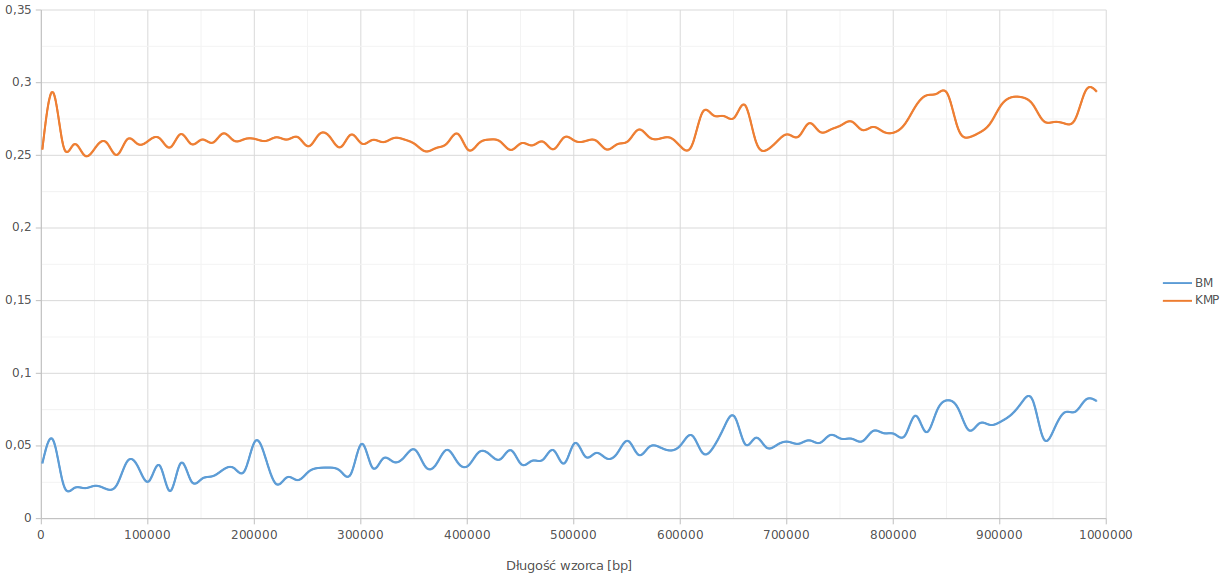
\includegraphics[width=1\textwidth]{img/kmp-vs-bm.png}
	\caption{\todo{opis - BMP vs KMP}}
	\label{img:kmp-vs-bm}
\end{figure}

\chapter{Podsumowanie}
\label{section:podsumowanie}

% \chapter{Opis algorytmów}
\label{ch:algorithms}



% \chapter{Implementacja}
\label{design}



% \chapter{Badania}
\label{section:badania}



% \chapter{Podsumowanie}
\label{summary}



\chapter*{Bibliografia}
\nocite{*}
\bibliographystyle{plplain}
%\bibliographystylebk{plplain}
%\bibliographystylest{plplain}
%\bibliographystyledoc{plplain}
% \bibliographystyleweb{plplain}
%\bibliographybk{BIB/books}
%\bibliographyst{BIB/books}
%\bibliographydoc{BIB/books}
% \bibliographyweb{BIB/books}

\bibliography{bib/mgr}

\appendix

%% \input{spis_rysunkow}

%% \input{spis_tabel}

%\input {spis_zalacznikow}

% \chapter{Instrukcje użytkownika}
\label{instructions}



\end{document}

% ex: set tabstop=4 shiftwidth=4 softtabstop=4 noexpandtab fileformat=unix filetype=tex spelllang=pl,en spell:

